\documentclass[10pt,letter]{article}
	% basic article document class
	% use percent signs to make comments to yourself -- they will not show up.

\usepackage{amsmath}
\usepackage{amssymb}
	% packages that allow mathematical formatting

\usepackage{graphicx}
	% package that allows you to include graphics

\usepackage{setspace}
	% package that allows you to change spacing

\onehalfspacing
	% text become 1.5 spaced

\usepackage{fullpage}
	% package that specifies normal margins
	
\usepackage[version=3]{mhchem} % Package for chemical equation typesetting
\usepackage{graphicx} % Required for the inclusion of images
\usepackage{natbib} % Required to change bibliography style to APA
\usepackage{amsmath} % Required for some math elements 
\usepackage{booktabs}
\usepackage{floatrow}
	

\begin{document}
	% line of code telling latex that your document is beginning


\title{CS 156 Problem Set 3}

\author{Christopher Zhen}

\date{Oct 17, 2016}
	% Note: when you omit this command, the current dateis automatically included
 
\maketitle 
	% tells latex to follow your header (e.g., title, author) commands.

\begin{align*}
\Delta G & = RT\textrm{ln}\frac{c_2}{c_1} + ZF\Delta V \\
\Delta G & = (1.986*10^{-3})(310)\textrm{ln}\frac{20}{0.1} + (1)(23.1)(0.07) \\
\Delta G & = 4.88 \textrm{kCal/mol}
\end{align*}

\section*{Problem 1}

\textbf{(B)} - Plugging in all the numerical values, we find the following equation that we need to solve for N in:

\begin{equation}
0.03 = 2*(1)*e^{-2 (0.05) ^{2} N}
\end{equation}

Solving for N, we get 839.9 which is closest to 1000.

\section*{Problem 2}

\textbf{(C)} - This time, we're solving:

\begin{equation}
0.03 = 2*(10)*e^{-2 (0.05) ^{2} N}
\end{equation}

And we get $N = 1300.5$ which is closest to 1500.

\section*{Problem 3} 

\textbf{(D)} - This time, we're solving:

\begin{equation}
0.03 = 2*(100)*e^{-2 (0.05) ^{2} N}
\end{equation}

And we get $N = 1761$ which is closest to 2000.

\section*{Problem 4}

\textbf{(B)} - Since to have a break point, we basically need to find a way to create planarly inseparable data (for 3 dimensions), all we need are the minimum number of points needed to define a plane (3) and two points on either side of the plane. This gives us 5 points required to have a break point.

\section*{Problem 5}

\textbf{(B)} - In order for something to be a valid growth function, it must have a break point $> 1$ since any data set with one point can be shattered regardless of what we use to classify it. Expression iii has a break point at $N=0$ and expression iv has as break point at $N=1$ so both of these are invalid. Expression i has as break point at 2 so it's okay; expression ii has a break point at 3 so it's okay; expression v has a break point at $\inf$ so it's okay.

\section*{Problem 6}

%\begin{figure}[H]
%\begin{center}
%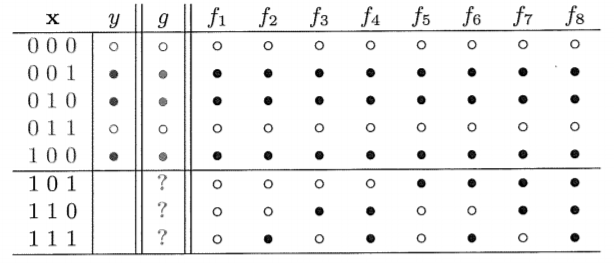
\includegraphics[width=0.75\textwidth]{FactorTable.PNG}
%\caption{Table courtesy of the textbook \textit{Learning from Data}.}
%\label{FactorTable}
%\end{center}
%\end{figure}

\textbf{(C)} - The easiest way to have a breakpoint with 2 intervals is if you have 5 alternating +1 and -1 points (starting with a +1). Alternatively, if you think about the case with 4 alternating +1 and -1 points (again starting with +1), this can be separated with 2 intervals, but the addition of the last +1 point breaks the separability.

\section*{Problem 7}

\textbf{(C)} - Using a similar "bins and balls" approach we tried in class for the 1 interval case, there are ${N+1}\choose{4}$ ways to choose 4 ends of the two intervals. We can then assign the first two ends to one interval and the other two to the second interval. Next we have to consider the case where the two ends of the interval are the same point, so we essentially have the "one interval" case and there are ${N+1}\choose{2}$ ways to arrange the endpoints. Finally, there is a final arrangement with no intervals that gives the $+ 1$ term.

\section*{Problem 8}

\textbf{(D)} - We already know that for $M = 1$, the smalles break point is with 3 points and when $M = 2$, we need 5 points. Therefore, for M intervals, we need $2M + 1$ points for a break point.

\section*{Problem 9}

\textbf{(D)} - Since we have 3 lines, we can properly classify $2*3+1 = 7$ points, so the largest possible set of n we can shatter is $n = 7$. We use this expression since we can always include 3 points in a triangle, so any number of points up to 7 can be shattered. Also if you think about 8 points around a circle, in order to classify every other point as +1, you need a rectangle (4 lines).

\section*{Problem 10}

\textbf{(B)} - This situation is similar to the single interval situation we went over in class because you're essentially picking both an inner and an outer boundary where the boundaries are radially symmetric.

\end{document}
	% line of code telling latex that your document is ending. If you leave this out, you'll get an error
